\section{Numerical simulations} \label{sec:numerics}

All the schemes we consider \revision{in this section} use the third order CWENOZ reconstruction without ghost cells, see~\cite{STP23:cweno:boundary}, described in Definition~\ref{def:CWENOZb} and \ref{def:CWENOZAO} with parameters $q=p=2$ in \eqref{eq:omegaZ} and
\begin{equation*}
	\begin{cases}
		d_L=\frac18, d_R=\frac18, & \text{for the inner computational cells} \\
		\tilde{d}=\max\{h,0.01\}, d=\frac14, & \text{for the first/last computational cell.}
	\end{cases}
\end{equation*}

For the purposes of this work it is sufficient to consider the very simple Rusanov (local Lax-Friedrichs) numerical flux
\begin{equation} \label{eq:lxf}
	\mathcal{F}(\mathbf{v},\mathbf{w}) = \frac12 \left( \mathbf{f}(\mathbf{v}) + \mathbf{f}(\mathbf{w}) - \alpha (\mathbf{w} - \mathbf{v}) \right), 
\end{equation}
with $\alpha = \max\{\|\mathbf{f}'(\mathbf{v})\|,\|\mathbf{f}'(\mathbf{w})\|\}$, where $\|\mathbf{f}'(\cdot)\|$ denotes the \revision{spectral radius} of the Jacobian of the flux function $\mathbf{f}$.
Furthermore, when assembling the Jacobian of $\mathbf{G}$ of \eqref{eq:predictor:system} for the Newton step \eqref{eq:predicor:newton},
we neglect the terms $\partial_{\mathbf{v}}\alpha$ and $\partial_{\mathbf{w}}\alpha$ in the derivative of $\mathcal{F}$ and approximate it as
\begin{equation*}
	\partial_{\mathbf{v}}\mathcal{F}(\mathbf{v},\mathbf{w}) 
	\approx \tfrac12 \mathrm{J}_{\mathbf{f}}(\mathbf{v}) 
	+ \tfrac12\alpha \mathbb{I}_m 
	\quad\text{and}\quad    
	\partial_{\mathbf{w}}\mathcal{F}(\mathbf{v},\mathbf{w}) 
	\approx \tfrac12 \mathrm{J}_{\mathbf{f}}(\mathbf{w}) 
	- \tfrac12\alpha \mathbb{I}_m,
\end{equation*}
where $\mathrm{J}_{\mathbf{f}}$ denotes the Jacobian of the exact flux function and $\mathbb{I}_m$ is the $m\times m$ identity matrix. \revision{For simplicity and not to distract from the main focus of the paper, which is on the implicit time integration of high order schemes, we have used the simple Rusanov flux. In fact, in~\eqref{eq:lxf} $\alpha$ is chosen as the maximum spectral radius of the Jacobian, namely as one would do with an explicit scheme. In implicit schemes this choice would deserve more attention, especially if the fluid speed is much lower than the sound speed and if one is not interested in the acoustic waves. In this case one can use different speed estimates in the approximate Riemann solver as explained in~\cite{2011DegondTang}.}

For the time integration, we employ the three stage third order DIRK scheme of~\cite{Alexander1977} with Butcher tableau
\begin{equation*}
	\setlength\arraycolsep{10pt}
	\begin{array}{c|ccc}
		\lambda & \lambda & 0 & 0 \\[1.5ex]
		\frac{(1+\lambda)}{2} & \frac{(1-\lambda)}{2} & \lambda & 0 \\[1.5ex]
		1 & -\frac32 \lambda^2 + 4\lambda - \frac14 & \frac32\lambda^2-5\lambda+\frac54 & \lambda \\[1ex]
		\hline
		&&&\\[-1.5ex]
		& -\frac32 \lambda^2 + 4\lambda - \frac14 & \frac32\lambda^2-5\lambda+\frac54 & \lambda
	\end{array}
\end{equation*}
where $\lambda=0.4358665215$. \revision{This method is A-stable and stiffly accurate, and therefore it is L-stable.} As a consequence, the Butcher tableau~\eqref{eq:tableau:be} of the composite backward Euler becomes
\begin{equation*}
	\setlength\arraycolsep{10pt}
	\begin{array}{c|ccc}
		\lambda & \lambda & 0 & 0 \\[1.5ex]
		\frac{(1+\lambda)}{2} & \lambda & \frac{1-\lambda}{2} & 0 \\[1.5ex]
		1 & \lambda & \frac{1-\lambda}{2} & \frac{1-\lambda}{2} \\[1ex]
		\hline
		&&&\\[-1.5ex]
		& \lambda & \frac{1-\lambda}{2} & \frac{1-\lambda}{2}
	\end{array}
\end{equation*}
Although this is not necessary for our construction, note that the sequence of the abscissae of this Runge-Kutta schemes is strictly increasing. Other choices of DIRK schemes are possible, e.g.~see~\cite{2009KetchesonMacdonaldGottlieb}.

\begin{table}[t]
	\caption{List of the schemes \revision{tested}, labels and line type (for those that appear in the plots)}
	\begin{center}
		\begin{tabular}{c|c|c}
			%\hline
			\underline{Label} & \underline{Scheme description} & \underline{Line type} \\[2ex]
			%\hline\hline
			$\Q$ & Quinpi solution without time-limiting & \begin{tikzpicture}\draw[green!50!black] (1,0)--(2,0);\node[green!50!black] at (1.5,0) {\pgfuseplotmark{*}};\end{tikzpicture} \\[2ex]
			$\QI{1}$ & Quinpi solution with $\mathcal{I}_1$ time-limiting strategy & 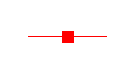
\begin{tikzpicture}\draw[red] (1,0)--(2,0);\node[red] at (1.5,0) {\pgfuseplotmark{square*}};\end{tikzpicture} \\[2ex]
			$\QI{2}$ & Quinpi solution with $\mathcal{I}_2$ time-limiting strategy & Not used%\begin{tikzpicture}\draw[magenta] (1,0)--(2,0);\node[magenta] at (1.5,0) {\pgfuseplotmark{diamond*}};\end{tikzpicture} 
			\\[2ex]
			$\QI{3}$ & Quinpi solution with $\mathcal{I}_3$ time-limiting strategy & \begin{tikzpicture}\draw[blue] (1,0)--(2,0);\node[blue] at (1.5,0) {\pgfuseplotmark{triangle*}};\end{tikzpicture} \\[2ex]
			$\Qexp$ & $\Q$ with CFL set as in explicit schemes & \begin{tikzpicture}\draw[dashed,green!50!black] (1,0)--(2,0);\node[green!50!black] at (1.5,0) {\pgfuseplotmark{o}};\end{tikzpicture} \\[2ex]
			$\QIexp{1}$ & $\QI{1}$ with CFL set as in explicit schemes & \begin{tikzpicture}\draw[dashed,red] (1,0)--(2,0);\node[red] at (1.5,0) {\pgfuseplotmark{square}};\end{tikzpicture} \\[2ex]
			$\QIexp{2}$ & $\QI{2}$ with CFL set as in explicit schemes & 
			Not used%\begin{tikzpicture}\draw[dashed,magenta] (1,0)--(2,0);\node[magenta] at (1.5,0) {\pgfuseplotmark{diamond}};\end{tikzpicture}
			\\[2ex]
			$\QIexp{3}$ & $\QI{3}$ with CFL set as in explicit schemes & \begin{tikzpicture}\draw[dashed,blue] (1,0)--(2,0);\node[blue] at (1.5,0) {\pgfuseplotmark{triangle}};\end{tikzpicture} \\[2ex]
			$\CW$ & Explicit CWENOZ scheme of~\cite{STP23:cweno:boundary} & \begin{tikzpicture}\draw[dashdotted,purple] (1,0)--(2,0);\node[purple] at (1.5,0) {\pgfuseplotmark{star}};\end{tikzpicture} \\[2ex]
			$\QP$ & Implicit scheme of~\cite{PSV23:Quinpi} & \begin{tikzpicture}\draw[pink] (1,0)--(2,0);\node[pink] at (1.5,0) {\pgfuseplotmark{diamond*}};\end{tikzpicture} \\[2ex]
			$\QPMOOD$ & Implicit scheme of~\cite{VTSP23:Quinpi:Book} & \begin{tikzpicture}\draw[gray] (1,0)--(2,0);\node[gray] at (1.5,0) {\pgfuseplotmark{diamond}};\end{tikzpicture} \\
			%\hline
		\end{tabular}
	\end{center}
	\label{tab:labels}
\end{table}

All numerical simulations are performed with the schemes described in Table~\ref{tab:labels}. For the time-limited schemes, we choose the threshold parameters in \eqref{eq:strategy1}, \eqref{eq:strategy2} and \eqref{eq:strategy3} as $\gamma_1 = h$, $\gamma_2 = 0.1$ and $\sigma = 10^{-10}$. \revision{The choices of the thresholds $\gamma_1$ and $\gamma_2$ are dictated by the decay of the numerical entropy indicators, cf.~Section~\ref{sec:quinpi:entropy:indicators}, and by the regions of the solution one aims to mark as irregular. Indeed, $\gamma_1=h$ allows us to mark as irregular all regions of the solution where $S^3 > h$, i.e.~those regions characterized by shock and contact waves, and rarefaction corners. Similarly, $\gamma_2=0.1$ allows us to distinguish smooth regions, where the indicator $\nicefrac{S^3}{S^1} \sim \mathcal{O}(h^2)$, from irregular regions where $\nicefrac{S^3}{S^1} \sim \mathcal{O}(1)$.}

For the solution of the nonlinear systems in the predictor and in the corrector, we used the Newton-Raphson schemes \eqref{eq:predicor:newton} and \eqref{eq:corrector:newton}, and a simple GMRES linear solver with a ILU0 preconditioner. For a detailed discussion on properties of iterative solvers in the context of implicit discretizations of hyperbolic equations we refer to~\cite{2022BirkenLinders}.

\subsection{Gas-dynamics problems} \label{sec:numerics:euler}

In this section, we test the third order Quinpi scheme on several problems based on the one-dimensional nonlinear Euler system for gas-dynamics
\begin{equation} \label{eq:euler:system}
	\partial_t 
	\left( \begin{array}{c}
		\rho \\ \rho v \\ E
	\end{array}\right) +
	\partial_x 
	\left( \begin{array}{c}
		\rho v \\ \rho v^2 + p \\ v(E+p)
	\end{array}\right)  = 0,
\end{equation}
where $\rho$, $v$, $p$ and $E$ are the density, velocity, pressure and energy per unit volume of an ideal gas, whose equation of state is $ E = \frac{p}{\gamma-1} + \frac12 \rho v^2, $ where $\gamma = 1.4$. The eigenvalues of the Jacobian of the flux are $\lambda_1 = v-c$, $\lambda_2=v$ and $\lambda_3=v+c$, where $c=\sqrt{\nicefrac{\gamma p}{\rho}}$ is the sound speed. For this system, we consider the entropy pair defined by the entropy function $\eta(\mathbf{u}) = -\rho \log\left(\frac{p}{(\gamma-1)\rho^\gamma}\right)$ and the entropy flux $\psi(\mathbf{u}) = -v\eta(\mathbf{u})$, see~\cite{GodlewskiRaviart96}.

\subsubsection{Convergence test}

We check the order of accuracy on the nonlinear system~\eqref{eq:euler:system} by simulating the advection of a density perturbation. The initial condition is
\begin{equation} \label{eq:conv:test:ic}
	\left(\rho,v,p\right) = \left(1+0.5\sin(2\pi x), 1, 1\right),
\end{equation}
so that the exact solution at a given time $t$ is a traveling wave
\begin{equation} \label{eq:conv:test:exact}
	\left(\rho,v,p\right) = \left(1+0.5\sin\left(2\pi (x-t)\right), 1, 1\right).
\end{equation}
We run the problem up to the final time $t=1$. \revision{We use periodic boundary conditions on the domain $[0,1]$ and, thus, we test not only the scheme accuracy, but also the proposed treatment of reconstructions for cells at the boundary.}

For this problem, the spectral radius is $\lambda_{\max} := \max_{i=1,2,3} |\lambda_i| \approx 2.67$, where $\lambda_i$ denotes the $i$-th eigenvalue of the system, which is preserved during the time evolution. For an explicit scheme the CFL stability condition would require to choose a grid ratio
$$
\frac{\DT}{h} \leq \frac{1}{\lambda_{\max}} \approx 0.37.
$$ 
In order to test the accuracy of the implicit scheme, we overcome the CFL condition running the simulation with the following grid ratios:
$$
\frac{\DT}{h} = 4, \quad \frac{\DT}{h} = 16,
$$
corresponding to the Courant numbers $C = \lambda_{\max}\tfrac{\DT}{h} \approx 10.7$ and $C \approx 41.8$, respectively.

The $L^1$- and $L^\infty$-norm errors computed on the density component and the corresponding experimental orders of convergence are listed in Table~\ref{tab:rates:cfl10} and Table~\ref{tab:rates:cfl40} for the two different Courant numbers.

While the schemes $\QI{1}$ and $\QI{3}$ achieve the theoretical order of convergence, the scheme $\QI{2}$ exhibits, instead, first order accuracy. This behavior is explained by investigating the time-limiting procedure for $\QI{2}$. In fact, \revision{the marking strategy $\mathcal{I}_2$ fails on flat regions where both $S^3$ and $S^1$ are floating point zeros. This} causes the limiting of all the numerical fluxes, and thus computed solution ends up coinciding with the first order predictor. Instead, the other detectors for time-limiting are able to signal the regularity of the solution, avoiding the \revision{unnecessary} activation of the time-limiting. For these reasons, in the following we will not consider the scheme $\QI{2}$ anymore.

\revision{Furthermore, we observe that Table~\ref{tab:rates:cfl10} and Table~\ref{tab:rates:cfl40} present identical errors and rates of convergence for the methods $\QI{1}$ and $\QI{3}$. This happens because the time-limiting is indeed off on the smooth profile: the two strategies detect no irregular cells and coincide with the unlimited scheme $\Q$.}

%\addtolength{\tabcolsep}{3pt}
\begin{table}[th!]
	\caption{Comparisons of the orders of convergence of Quinpi schemes with Courant number $C=10.7$.\label{tab:rates:cfl10}}
	\centering
	\vspace{0.25cm}
	\pgfplotstabletypeset[
	font=\small,
	col sep=comma,
	sci zerofill,
	empty cells with={--},
	every head row/.style={before row={\toprule
			&\multicolumn{2}{c}{$\QI{1}$}
			&\multicolumn{2}{c}{$\QI{2}$}
			&\multicolumn{2}{c}{$\QI{3}$}
			\\
		},
		after row=\midrule
	},
	every last row/.style={after row=\bottomrule},
	create on use/rate1/.style={create col/dyadic refinement rate={1}},
	create on use/rate2/.style={create col/dyadic refinement rate={2}},
	create on use/rate3/.style={create col/dyadic refinement rate={3}},
	columns/0/.style={column name={$N$}},
	columns/1/.style={column name={$L^1$ error}},
	columns/rate1/.style={fixed zerofill,column name={rate}},
	columns/2/.style={column name={$L^1$ error}},
	columns/rate2/.style={fixed zerofill,column name={rate}},
	columns/3/.style={column name={$L^1$ error}},
	columns/rate3/.style={fixed zerofill,column name={rate}},
	columns={0,1,rate1,2,rate2,3,rate3},
	%skip rows between index={0}{2}
	]
	{dtdx4_err1.err}
	\\
	\vspace{0.25cm}
	\pgfplotstabletypeset[
	font=\small,
	col sep=comma,
	sci zerofill,
	empty cells with={--},
	every head row/.style={before row={\toprule
			&\multicolumn{2}{c}{$\QI{1}$}
			&\multicolumn{2}{c}{$\QI{2}$}
			&\multicolumn{2}{c}{$\QI{3}$}
			\\
		},
		after row=\midrule
	},
	every last row/.style={after row=\bottomrule},
	create on use/rate1/.style={create col/dyadic refinement rate={1}},
	create on use/rate2/.style={create col/dyadic refinement rate={2}},
	create on use/rate3/.style={create col/dyadic refinement rate={3}},
	columns/0/.style={column name={$N$}},
	columns/1/.style={column name={$L^\infty$ error}},
	columns/rate1/.style={fixed zerofill,column name={rate}},
	columns/2/.style={column name={$L^\infty$ error}},
	columns/rate2/.style={fixed zerofill,column name={rate}},
	columns/3/.style={column name={$L^\infty$ error}},
	columns/rate3/.style={fixed zerofill,column name={rate}},
	columns={0,1,rate1,2,rate2,3,rate3},
	%skip rows between index={0}{2}
	]
	{dtdx4_errinf.err}
\end{table}

\begin{table}[th!]
	\caption{Comparisons of the orders of convergence of Quinpi schemes with Courant number $C=41.8$.\label{tab:rates:cfl40}}
	\centering
	\vspace{0.25cm}
	\pgfplotstabletypeset[
	font=\small,
	col sep=comma,
	sci zerofill,
	empty cells with={--},
	every head row/.style={before row={\toprule
			&\multicolumn{2}{c}{$\QI{1}$}
			&\multicolumn{2}{c}{$\QI{2}$}
			&\multicolumn{2}{c}{$\QI{3}$}
			\\
		},
		after row=\midrule
	},
	every last row/.style={after row=\bottomrule},
	create on use/rate1/.style={create col/dyadic refinement rate={1}},
	create on use/rate2/.style={create col/dyadic refinement rate={2}},
	create on use/rate3/.style={create col/dyadic refinement rate={3}},
	columns/0/.style={column name={$N$}},
	columns/1/.style={column name={$L^1$ error}},
	columns/rate1/.style={fixed zerofill,column name={rate}},
	columns/2/.style={column name={$L^1$ error}},
	columns/rate2/.style={fixed zerofill,column name={rate}},
	columns/3/.style={column name={$L^1$ error}},
	columns/rate3/.style={fixed zerofill,column name={rate}},
	columns={0,1,rate1,2,rate2,3,rate3},
	skip rows between index={0}{3}
	]
	{dtdx16_err1.err}
	\\
	\vspace{0.25cm}
	\pgfplotstabletypeset[
	font=\small,
	col sep=comma,
	sci zerofill,
	empty cells with={--},
	every head row/.style={before row={\toprule
			&\multicolumn{2}{c}{$\QI{1}$}
			&\multicolumn{2}{c}{$\QI{2}$}
			&\multicolumn{2}{c}{$\QI{3}$}
			\\
		},
		after row=\midrule
	},
	every last row/.style={after row=\bottomrule},
	create on use/rate1/.style={create col/dyadic refinement rate={1}},
	create on use/rate2/.style={create col/dyadic refinement rate={2}},
	create on use/rate3/.style={create col/dyadic refinement rate={3}},
	columns/0/.style={column name={$N$}},
	columns/1/.style={column name={$L^\infty$ error}},
	columns/rate1/.style={fixed zerofill,column name={rate}},
	columns/2/.style={column name={$L^\infty$ error}},
	columns/rate2/.style={fixed zerofill,column name={rate}},
	columns/3/.style={column name={$L^\infty$ error}},
	columns/rate3/.style={fixed zerofill,column name={rate}},
	columns={0,1,rate1,2,rate2,3,rate3},
	skip rows between index={0}{3}
	]
	{dtdx16_errinf.err}
\end{table}

\subsubsection{Stiff Riemann problems}

In the following, we test Quinpi schemes on stiff Riemann problems for the Euler system~\eqref{eq:euler:system}, namely for those problems characterized by $\frac{|v|}{|v|+c} \ll 1, \quad \forall\,(x,t)$.
In this case, we expect a strong separation between acoustic and material waves, because they travel with speeds having different magnitudes. In particular, the acoustic speeds would impose a strict constraint on the time-step
$$
\frac{\DT_{\text{stab}}}{h} \leq \frac{1}{\max_{x} |v|+c}.
$$
With implicit schemes, instead, the time-step is not dictated by stability and therefore we will choose it in order to reproduce accurately the slow material wave:
$$
\frac{\DT_{\text{acc}}}{h} = \frac{1}{|v_{\text{cw}}|},
$$
where $v_{\text{cw}}$ denotes the \revision{velocity} of the contact wave. The ratio between the time-step $\DT_{\text{stab}}$ required for stability and the time-step $\DT_{\text{acc}}$ required for accuracy on the material wave, is a measure of the stiffness of the problem. The Courant number is thus
$$
C = \frac{\DT_{\text{acc}}}{\Delta t_{\text{stab}}}.
$$


% Figure environment removed

We consider the following Riemann problems.

\begin{description}
	\item[Test (a): symmetric expansion problem.]
	\begin{equation} \label{eq:tworar:ic}
		\left(\rho,u,p\right) = \begin{cases}
			(1, -0.15, 1), & x < 0\\
			(0.5,0.15,1), & x \geq 0.
		\end{cases}
	\end{equation}
	The exact \revision{density} solution at time $t=1$ is depicted in the left panel of Figure~\ref{fig:exact} and is characterized by a 1-rarefaction moving with negative \revision{velocity}, a 3-rarefaction moving with positive \revision{velocity}, and a 2-contact wave with \revision{velocity} $v_{\text{cw}}=-2.57\cdot10^{-2}$.
	For this problem, one has
	$
	\max_{(x,t)} |v|+c = 1.82, %\ \text{ and } \ 3.8\cdot10^{-4} \leq \mathrm{Ma} \leq 0.17.
	$
	thus an explicit scheme would require to choose a time-step $\DT_{\text{stab}}$ such that
	$$
	\frac{\DT_{\text{stab}}}{h} \leq 0.549.
	$$
	With an implicit scheme, it is possible to overcome this stability restriction. In particular, choosing a time-step $\DT_{\text{acc}}$ to meet the accuracy on the contact wave, one has
	$$
	\frac{\DT_{\text{acc}}}{h} = 6.66,
	$$
	which implies a Courant number $C \approx 12.1$.
	
	\item[Test (b): colliding flow problem.]
	\begin{equation} \label{eq:twoshocks:ic}
		\left(\rho,v,p\right) = \begin{cases}
			(1.5,  0.5, 10), & x < 0\\
			(0.5, -0.5, 10), & x \geq 0.
		\end{cases}
	\end{equation}
	The exact \revision{density} solution at time $t=1$ is depicted in the center panel of Figure~\ref{fig:exact} and is characterized by a 1-shock wave moving with negative \revision{velocity}, a 3-shock wave moving with positive \revision{velocity}, and a 2-contact wave with \revision{velocity} $v_{\text{cw}}=0.13$.
	For this problem, one has
	$
	\max_{(x,t)} |v|+c = 5.79, %\ \text{ and } \ 2.5\cdot10^{-2} \leq \mathrm{Ma} \leq 0.16.
	$
	thus an explicit scheme would require to choose a time-step $\DT_{\text{stab}}$ such that
	$$
	\frac{\DT_{\text{stab}}}{h} \leq 0.17.
	$$
	With an implicit scheme, instead, one can choose
	$$
	\frac{\DT_{\text{acc}}}{h} = 2,
	$$
	which implies a Courant number $C \approx 11.6$.
	
	\item[Test (c): modified Lax shock tube problem.] \begin{equation} \label{eq:stiffLax:ic}
		\left(\rho,v,p\right) = \begin{cases}
			(0.445,  0, 3.528), & x < 0\\
			(0.5, 0, 2.528), & x \geq 0.
		\end{cases}
	\end{equation}
	\revision{Compared to the classical Lax shock tube problem, the initial condition is characterized by a zero left velocity and a higher right pressure. This allows a faster separation of the waves.} The exact \revision{density} solution at time $t=0.15$ is depicted in the right panel of Figure~\ref{fig:exact} and is characterized by a 1-rarefaction moving with negative \revision{velocity}, a 3-shock moving with positive \revision{velocity}, and a 2-contact wave with \revision{velocity} $v_{\text{cw}}=0.35$.
	For this problem, one has
	$
	\max_{(x,t)} |v|+c = 3.61,
	$
	thus an explicit scheme would require to choose a time-step $\DT_{\text{stab}}$ such that
	$$
	\frac{\DT_{\text{stab}}}{h} \leq 0.28.
	$$
	With an implicit scheme, instead, one can choose
	$$
	\frac{\DT_{\text{acc}}}{h} = 2.83,
	$$
	which implies a Courant number $C \approx 10.2$.
\end{description}

% Figure environment removed

% Figure environment removed

% Figure environment removed

\begin{table}[t!]
	\caption{Statistics on the time-limiting procedure of Quinpi schemes. \revision{These data are graphically depicted in Figure~\ref{fig:xt:timelim}.}\label{tab:stat}}
	\begin{subtable}[h]{\textwidth}
		\caption{Symmetric expansion problem.\label{tab:stat:tworar}}
		\centering
		\vspace{0.25cm}
		\pgfplotstabletypeset[
		font=\footnotesize,
		col sep=comma,
		sci zerofill,
		empty cells with={--},
		every head row/.style={before row={\toprule
				&\multicolumn{2}{c}{$\QI{3}$}&\multicolumn{2}{c}{$\QIexp{3}$}
				\\[2ex]
			},
			after row=\midrule
		},
		every last row/.style={after row=\bottomrule},
		columns/0/.style={column name={$N$}},
		columns/4/.style={column name={\shortstack{max.~number of \\ limited fluxes}}},
		columns/5/.style={column name={\shortstack{\% limited \\ time-steps}}},
		columns/9/.style={column name={\shortstack{max.~number of \\ limited fluxes}}},
		columns/10/.style={column name={\shortstack{\% limited \\ time-steps}}},
		columns={0,4,5,9,10},%,6,7,8,9,10,11,12,13,14,15},
	%skip rows between index={0}{2}
	]
	{ind313_stat_tworar.out}
\end{subtable}
\begin{subtable}[h]{\textwidth}
	\vspace{0.25cm}
	\caption{Colliding flows problem.\label{tab:stat:twoshocks}}
	\centering
	\vspace{0.25cm}
	\pgfplotstabletypeset[
	font=\footnotesize,
	col sep=comma,
	sci zerofill,
	empty cells with={--},
	every head row/.style={before row={\toprule
			&\multicolumn{2}{c}{$\QI{3}$}&\multicolumn{2}{c}{$\QIexp{3}$}
			\\[2ex]
		},
		after row=\midrule
	},
	every last row/.style={after row=\bottomrule},
	columns/0/.style={column name={$N$}},
	columns/4/.style={column name={\shortstack{max.~number of \\ limited fluxes}}},
	columns/5/.style={column name={\shortstack{\% limited \\ time-steps}}},
	columns/9/.style={column name={\shortstack{max.~number of \\ limited fluxes}}},
	columns/10/.style={column name={\shortstack{\% limited \\ time-steps}}},
	columns={0,4,5,9,10},%,6,7,8,9,10,11,12,13,14,15},
%skip rows between index={0}{2}
]
{ind313_stat_twoshocks.out}
\end{subtable}
\begin{subtable}[h]{\textwidth}
\vspace{0.25cm}
\caption{Modified Lax's problem.\label{tab:stat:stiffLax}}
\centering
\vspace{0.25cm}
\pgfplotstabletypeset[
font=\footnotesize,
col sep=comma,
sci zerofill,
empty cells with={--},
every head row/.style={before row={\toprule
		&\multicolumn{2}{c}{$\QI{3}$}&\multicolumn{2}{c}{$\QIexp{3}$}
		\\[2ex]
	},
	after row=\midrule
},
every last row/.style={after row=\bottomrule},
columns/0/.style={column name={$N$}},
columns/4/.style={column name={\shortstack{max.~number of \\ limited fluxes}}},
columns/5/.style={column name={\shortstack{\% limited \\ time-steps}}},
columns/9/.style={column name={\shortstack{max.~number of \\ limited fluxes}}},
columns/10/.style={column name={\shortstack{\% limited \\ time-steps}}},
columns={0,4,5,9,10},%,6,7,8,9,10,11,12,13,14,15},
%skip rows between index={0}{2}
]
{ind313_stat_stiffLax.out}
\end{subtable}
\end{table}

% Figure environment removed

% % Figure environment removed

Here below we comment on the results of all three tests.
First we show the need for time-limiting. In Figure~\ref{fig:timelim} we compare the solutions computed without time-limiting ($\Q$) an with the two limiting strategies $\mathcal{I}_1$ and $\mathcal{I}_3$. The figures clearly show that
\begin{itemize}
\item time-limiting is needed to avoid spurious oscillations;
\item strategy $\mathcal{I}_1$, see~\eqref{eq:strategy1}, is more diffusive. Therefore, in the following we will consider the third strategy $\mathcal{I}_3$ only, see~\eqref{eq:strategy3}.
\end{itemize}

Next, we study the effect of the choice of time-step. Schemes $\Qexp$ and $\QIexp{3}$ are obtained with a time-step $\DT=\DT_{\text{stab}}$, instead schemes $\Q$ and $\QI{3}$ are obtained with a time-step $\DT=\DT_{\text{acc}}$, i.e.~centered on the material wave. In Figure~\ref{fig:implicit} we show the results and we observe that
\begin{itemize}
\item on the contact wave, which is the one that we wish to focus on, all schemes are similarly accurate despite the fact that schemes $\Q$ and $\QI{3}$ run with a time-step that is about $10$ times larger;
\item schemes $\Qexp$ and $\QIexp{3}$, as expected, are more accurate on the acoustic waves than the schemes $\Q$ and $\QI{3}$;
\item time-limiting is needed also when $\DT=\DT_{\text{stab}}$, as can be observed also in Figure~\ref{fig:xt:timelim} and in Table~\ref{tab:stat}. \revision{In particular, in Figure~\ref{fig:xt:timelim} it is evident that the time-limiting is active on all the waves at initial times, i.e.~when they separate themselves. At larger times, instead, limiting acts in particular on shock waves but only intermittently during the evolution.} \revision{In Table~\ref{tab:stat} we observe that the percentage of limited steps is larger when $\DT=\DT_{\text{acc}}$ but in this case the number of time-steps is roughly $10$ times smaller. Moreover, the number of limited fluxes is larger when $\DT=\DT_{\text{acc}}$ because a wave propagates across more cells in a single time-step compared to the case when $\DT=\DT_{\text{stab}}$.}
\end{itemize}

Now we compare the explicit scheme \cite{STP23:cweno:boundary}, which has to be run with $\DT_{\text{stab}}$, and the implicit scheme run at $\DT_{\text{acc}}$.
Figure~\ref{fig:imex} shows that
\begin{itemize}
\item on the contact wave, which is the one we are focusing on, all schemes are similarly accurate on all tests;
\item as expected, the explicit scheme is more accurate than the implicit one on the acoustic waves.
\end{itemize}

\subsection{Low-Mach problems} \label{sec:numerics:lowMach}

In this section, we test the performance of Quinpi schemes on low-Mach problems, namely such that
$$
\mathrm{Ma} := \frac{|v|}{c} \ll 1, \quad \forall\,(x,t).
$$
Here, the aim is to show that the implicit framework we propose has the ability to \revision{guarantee stability and accuracy} on such problems. We do not claim that the Quinpi approach is asymptotic preserving, e.g.~see~\cite{2017DimarcoLoubereVignal}.

In order to describe the low-Mach number limit, we consider the rescaled compressible Euler system
\begin{equation} \label{eq:euler:system:rescaled}
\partial_t 
\left( \begin{array}{c}
\rho \\ \rho v \\ E
\end{array}\right) +
\partial_x 
\left( \begin{array}{c}
\rho v \\ \rho v^2 + \frac{1}{\varepsilon^2} p \\ v(E+p)
\end{array}\right)  = 0,
\end{equation}
with the equation of state $E = \frac{p}{\gamma-1} + \frac{\varepsilon^2}{2} \rho v^2$, $\gamma=1.4$.
The parameter $\varepsilon$ describes the Mach number within the non-dimensionalized system, and one has $\mathrm{Ma} = \nicefrac{\varepsilon}{\sqrt{\gamma}}$. System~\eqref{eq:euler:system:rescaled} is hyperbolic with eigenvalues $\lambda_1 = v - \nicefrac{c}{\varepsilon}$, $\lambda_2 = v$, $\lambda_3= v + \nicefrac{c}{\varepsilon}$.
For a more detailed discussion on the low-Mach number scaling we refer, e.g., to~\cite{2018BoscarinoRussoScandurra,1995Klein}.

\subsubsection{Convergence test}

We compute the experimental order of convergence of the Quinpi scheme on the computational domain [-2.5,2.5] using the smooth initial condition~\cite{2018BoscarinoRussoScandurra}
$$
\rho(x,0) = \left( 1 + \varepsilon \frac{(\gamma-1) u(x,0)}{2\sqrt{\gamma}} \right)^{\frac{2}{\gamma-1}}, \quad u(x,0) = \sin\left(\frac{2\pi x}{5}\right), \quad p(x,0) = \rho(x,0)^\gamma.
$$
The order of accuracy of the scheme is investigated at final time $t=0.3$ for $\varepsilon_1 = 0.8$, $\varepsilon_2=0.3$, and at final time $t=0.01$ for $\varepsilon_3=10^{-4}$. For this problem, $|v| \leq 1$, $\forall\,(x,t)$, and $\lambda_{\max}(\varepsilon) := \max_{(x,t)} |v|+\nicefrac{c}{\varepsilon}$ is
$$
\lambda_{\max}(0.8) = 2.6786, \quad \lambda_{\max}(0.3)=5.1439, \quad \lambda_{\max}(10^{-4})=1.1833 \cdot 10^{4}.
$$
For an explicit scheme the CFL stability condition would require to choose a grid ratio
\begin{align*}
\frac{\DT_{\varepsilon_1}}{h} &\leq \frac{1}{\lambda_{\max}(0.8)} \approx 0.3733, \\ \frac{\DT_{\varepsilon_2}}{h} &\leq \frac{1}{\lambda_{\max}(0.3)} \approx 0.1944, \\ \frac{\DT_{\varepsilon_3}}{h} &\leq \frac{1}{\lambda_{\max}(10^{-4})} \approx 8.45\cdot 10^{-5}.
\end{align*}
We overcome the CFL condition running the simulation using the following grid ratios:
$$
\frac{\DT_{\varepsilon_i}}{h} = \frac{C}{\lambda_{\max}(\varepsilon_i)}, \quad i=1,2,3,
$$
with Courant number $C = 20$.

\begin{table}[th!]
\caption{Experimental order of convergence of Quinpi scheme on the low-Mach problem with Courant number $C=20$.\label{tab:ratesLM:cfl20}}
\centering
\vspace{0.25cm}
\pgfplotstabletypeset[
font=\small,
col sep=comma,
sci zerofill,
empty cells with={--},
every head row/.style={before row={\toprule
&\multicolumn{2}{c}{$\varepsilon=0.8$}
&\multicolumn{2}{c}{$\varepsilon=0.3$}
&\multicolumn{2}{c}{$\varepsilon=10^{-4}$}
\\
},
after row=\midrule
},
every last row/.style={after row=\bottomrule},
create on use/rate1/.style={create col/dyadic refinement rate={1}},
create on use/rate2/.style={create col/dyadic refinement rate={2}},
create on use/rate3/.style={create col/dyadic refinement rate={3}},
columns/0/.style={column name={$N$}},
columns/1/.style={column name={$L^1$ error}},
columns/rate1/.style={fixed zerofill,column name={rate}},
columns/2/.style={column name={$L^1$ error}},
columns/rate2/.style={fixed zerofill,column name={rate}},
columns/3/.style={column name={$L^1$ error}},
columns/rate3/.style={fixed zerofill,column name={rate}},
columns={0,1,rate1,2,rate2,3,rate3},
skip rows between index={0}{3}
]
{err1.err}
\\
\vspace{0.25cm}
\pgfplotstabletypeset[
font=\small,
col sep=comma,
sci zerofill,
empty cells with={--},
every head row/.style={before row={\toprule
&\multicolumn{2}{c}{$\varepsilon=0.8$}
&\multicolumn{2}{c}{$\varepsilon=0.3$}
&\multicolumn{2}{c}{$\varepsilon=10^{-4}$}
\\
},
after row=\midrule
},
every last row/.style={after row=\bottomrule},
create on use/rate1/.style={create col/dyadic refinement rate={1}},
create on use/rate2/.style={create col/dyadic refinement rate={2}},
create on use/rate3/.style={create col/dyadic refinement rate={3}},
columns/0/.style={column name={$N$}},
columns/1/.style={column name={$L^\infty$ error}},
columns/rate1/.style={fixed zerofill,column name={rate}},
columns/2/.style={column name={$L^\infty$ error}},
columns/rate2/.style={fixed zerofill,column name={rate}},
columns/3/.style={column name={$L^\infty$ error}},
columns/rate3/.style={fixed zerofill,column name={rate}},
columns={0,1,rate1,2,rate2,3,rate3},
skip rows between index={0}{3}
]
{errinf.err}
\end{table}

Density errors for the different values of the Mach number are listed in Table~\ref{tab:ratesLM:cfl20} and computed with the Quinpi scheme $\Q$. The theoretical third order of convergence is observed.

\subsubsection{Two colliding acoustic pulses}

We consider the two colliding acoustic pulses taken from~\cite{1995Klein}. The initial condition is given by
\begin{align*}
\rho(x,0) &= \rho_0 + \frac{\varepsilon\rho_1}{2} \left( 1-\cos\left( \frac{2\pi x}{L} \right) \right), \quad \rho_0=0.955, \quad \rho_1=2, \\
u(x,0) &= -\frac{u_0}{2} \mathrm{sign}(x) \left( 1-\cos\left( \frac{2\pi x}{L} \right) \right), \quad u_0=2\sqrt{\gamma}, \\
p(x,0) &= p_0 + \frac{\varepsilon p_1}{2} \left( 1-\cos\left( \frac{2\pi x}{L} \right) \right), \quad p_0=1, \quad p_1=2\gamma,
\end{align*}
on the computational domain $[-L,L]$, $L=\nicefrac{2}{\varepsilon}$. \revision{We use periodic boundary conditions and, thus, we also test the proposed treatment of reconstructions for cells at the boundary.}

We choose $\varepsilon_1=\nicefrac{1}{11}$ and $\varepsilon_2=10^{-4}$. In both cases, $\max_{(x,t)} |v| = 2.3656$, whereas $\lambda_{\max}(\varepsilon_1) = 16.038$ and $\lambda_{\max}(\varepsilon_2) = 1.21\cdot 10^4$. Therefore, using an explicit scheme would require to choose a time-step
$$
\frac{\DT_{\varepsilon_1}}{h} \leq 6.24\cdot 10^{-2}, \quad \frac{\DT_{\varepsilon_2}}{h} \leq 8.26 \cdot 10^{-5}.
$$
With an implicit scheme, instead, we can choose
$$
\frac{\DT_{\varepsilon_1}}{h} = \frac{1}{\max_{(x,t)} |v|} = 4.23 \cdot 10^{-1},
$$
which corresponds to a Courant number $C = 6.78$. We employ the same Courant number for $\varepsilon_2$ which determines
$$
\frac{\DT_{\varepsilon_2}}{h} = 5.59 \cdot 10^{-4}.
$$

% Figure environment removed

In Figure~\ref{fig:colliding:pulses} we show the pressure profile obtained using the third order Quinpi scheme $\Q$ without time-limiting at final times $t = 0.815$ and $t = 1.63$, with $N=440$ cells. The solution is compared with the third order explicit scheme $\CW$.

\subsection{Scalar problems} \label{sec:numerics:scalar}

\revision{
Finally, we provide some numerical simulations on scalar conservation laws. In fact, although this work is mostly focused on hyperbolic systems, the Quinpi framework introduced in~\cite{PSV23:Quinpi}, and further extended in~\cite{VTSP23:Quinpi:Book}, was based on very different time-limiting procedures. Therefore, this section is aimed to investigate the performance of the proposed MOOD limiter combined with the numerical entropy production indicator on standard scalar problems.
}

\subsubsection{Linear transport}

\revision{
We consider the linear scalar conservation law
\begin{equation} \label{eq:linadv}
\partial_t u(x,t) + \partial_x u(x,t) = 0,
\end{equation}
\revision{for} $(x,t)\in[-1,1]\times(0,2]$, with periodic boundary conditions in space and discontinuous initial conditions:
\begin{subequations}\label{eq:nonsmoothIC}
\begin{equation} \label{eq:sindiscontIC}
u_0(x) = \sin(\pi x) +
\begin{cases}
	3, & -0.4 \leq x \leq 0.4,\\
	0, & \text{otherwise,}	
\end{cases}
\end{equation}
\begin{equation} \label{eq:doublestepIC}
u_0(x) =
\begin{cases}
	1, & -0.25 \leq x \leq 0.25,\\
	0, & \text{otherwise.}
\end{cases}
\end{equation}
\end{subequations}
Here, we consider the entropy function $\eta(u) = \frac{u^2}{2}$ and the entropy flux $\psi(u) = \frac{u^2}{2}$.
}

% Figure environment removed

\revision{
The results are reported in Figure~\ref{fig:lintra}, computed with two different Courant numbers, i.e.~$\nicefrac{\Delta t}{h}=5$ and $\nicefrac{\Delta t}{h}=10$ on $400$ space cells. As introduced in Table~\ref{tab:labels}, the solution labeled by $\QP$ refers to the scheme of~\cite{PSV23:Quinpi}, whereas the solution labeled by $\QPMOOD$ refers to the one of~\cite{VTSP23:Quinpi:Book}. We note that the scheme $\QI{3}$ performs better than the other two implicit schemes on the discontinuous sinusoidal profile since it produces lower dissipation around the jump discontinuities. However, the low-dissipation properties leads to lightly larger oscillations around the discontinuities of the double-step profile. In particular, with $\nicefrac{\Delta t}{h} = 10$, the upper flat part of the solution is not reproduced by all the schemes.
}

\subsubsection{Burgers' equation}

\revision{
Next, we compare the schemes on the nonlinear Burgers' equation
\begin{equation} \label{eq:burgers}
\partial_t u(x,t) + \partial_x \left( \frac{u^2(x,t)}{2} \right) = 0,
\end{equation}
\revision{for} $x\in[-1,1]$, with periodic boundary conditions in space. Here, we consider the entropy function $\eta(u) = \frac{u^2}{2}$ and the entropy flux $\psi(u) = \frac{u^3}{3}$.
}

% Figure environment removed

\revision{
First, we consider the discontinuous initial condition~\eqref{eq:doublestepIC} and compute the numerical solution at time $t=0.5$ on $400$ space cells with three different Courant numbers, i.e.~$\nicefrac{\Delta t}{h}=3,5,10$. The exact solution is characterized by a standing-tail with right-moving head rarefaction and a shock with positive \revision{velocity}. The results are reported in Figure~\ref{fig:burgers:doublestep}. We observe that the scheme $\QPMOOD$ reproduces the rarefaction and the shock with less dissipation when $\nicefrac{\Delta t}{h}=3$. However, the time-limiting of $\QPMOOD$ leads to higher dissipation at increasing Courant numbers. Moreover, while the dissipation of $\QP$ is lower than the dissipation of the other schemes on the rarefaction head at $\nicefrac{\Delta t}{h}=3$, we notice that $\QI{3}$ reproduces accurately the tail of the rarefaction and avoids the undershoot on the shock wave.
}

\revision{
Furthermore, we test the Burgers' equation on the smooth initial condition
\begin{equation} \label{eq:shockinteractionIC}
u_0(x) = 0.2 -\sin(\pi x) + \sin(2 \pi x), 
\end{equation}
computing the solution at three different times, namely $t=\nicefrac{1}{2\pi},0.6,1$, and Courant numbers $\nicefrac{\Delta t}{h}=3,10$, on a space grid of $400$ cells. The exact solution is characterized by the formation of two shocks which collide developing a single discontinuity.
}

% Figure environment removed

\revision{
The numerical results are depicted in Figure~\ref{fig:burgers:shockinteraction}. We observe that all schemes do not produce spurious oscillations at time $t=1/2\pi$, just before the two shocks appear, but the scheme $\QP$ is more diffusive. At $t=0.6$, $\QPMOOD$ exhibits a small undershoot on the left shock, clearly visible in the zoom box, which is not present in the solution computed by $\QI{3}$. Increasing the Courant number produces more dissipation within the numerical schemes $\QP$ and $\QPMOOD$, whereas $\QI{3}$ is more accurate and does not exhibit spurious oscillations.
}